\documentclass[twocolumn]{article}

\usepackage[margin=0.68in,columnsep=0.22in]{geometry}
\usepackage[T1]{fontenc}
\usepackage{amsmath}
\usepackage{amssymb}
\usepackage{booktabs}
\usepackage{graphicx}
\usepackage{array}
\usepackage[numbers,sort&compress]{natbib}

\graphicspath{{figures/}}
\setlength{\tabcolsep}{3.2pt}
\renewcommand{\arraystretch}{1.05}
\setlength{\parindent}{1em}
\setlength{\parskip}{0pt}

\title{When MRI Slice Interpolators Disagree:\
Ground-Truth-Free Reliability Assessment Across Models and Datasets}
\author{Anonymous Authors}
\date{}

\begin{document}
\maketitle

\begin{abstract}
Deep models for through-plane MRI interpolation are commonly judged by average reconstruction fidelity, although deployment requires deciding whether an individual synthetic slice or examination is trustworthy without observing its missing target. We study this gap as a ground-truth-free reliability-ranking problem. For a target reconstructor, we define a pixel-wise score as the median absolute deviation between its prediction and a heterogeneous committee of alternative interpolators. The score is computed from reconstruction outputs alone; reference targets are used only for evaluation. We test four reconstructors on IXI T2 and three on fastMRI-brain T2 and an external NingXia T2 cohort, totaling 161 examinations and ten fixed target--dataset evaluations. Foreground pixel error correlation ranges from 0.277 to 0.519 and examination-level Spearman correlation from 0.890 to 0.966. Normalized AURC is 0.024--0.092, and referring the highest-score half of examinations reduces retained MAE by 19.3--52.1\% relative to random review. Composition analyses show that neural peers are strongest on fastMRI, analytical references on NingXia, and neither is universally sufficient. The protocol is therefore a useful quality-control layer for existing interpolators, not a calibrated probability model or a replacement for clinical validation.
\end{abstract}

\section{Introduction}

Through-plane interpolation converts sparsely sampled MRI volumes into denser stacks and can support visualization, registration, and downstream volumetric analysis. Recent neural methods model inter-slice structure explicitly \citep{song2024i3net}, while restoration transformers provide strong generic image priors \citep{liang2021swinir,chen2022hat}. Their evaluation, however, is dominated by cohort-level averages such as PSNR, SSIM, and MAE. These averages answer whether a reconstructor is accurate on a test set; they do not tell an operator which synthetic examination should be reviewed.

This distinction matters because the missing slice is unavailable when the reconstruction is used. A high-error output can remain visually plausible, and a model with favorable mean fidelity may still fail on unusual anatomy, motion, contrast, or field-of-view. Learned uncertainty heads, Bayesian approximations, and repeated stochastic inference can expose some of this uncertainty \citep{gal2016dropout,kendall2017uncertainties,lakshminarayanan2017deepensembles}, but they require model access, retraining, or additional inference. In many retrospective studies, by contrast, predictions from several established reconstructors already coexist. Their disagreement is observable even when the target is not.

We therefore ask a deliberately operational question: \emph{can disagreement among heterogeneous slice interpolators rank reconstruction risk without access to the missing target?} We treat the output of one reconstructor as the target prediction and all other available outputs as a committee. A robust pixel-wise deviation yields a spatial reliability map; foreground aggregation yields an examination score. Ground truth enters only after scoring, to measure error association and selective-review utility.

This framing differs from calling ensemble variance a calibrated uncertainty distribution. The committee members are heterogeneous algorithms rather than posterior samples, and they can share errors. Our claims are consequently about \emph{ranking}: whether larger disagreement tends to coincide with larger error and whether referring high-score examinations lowers risk among retained cases.

Our contributions are threefold. First, we formulate ground-truth-free reliability assessment for MRI slice interpolation and provide a target-specific committee score whose implementation excludes the target from its reference set. Second, we evaluate spatial localization and examination-level selective risk across four reconstructors and three T2 MRI cohorts, including an external cross-validation cohort. Third, we stress-test the result with analytical-only and neural-only committees, score-level leave-one-member-out analysis, residual and shared-dispersion comparators, foreground masking, test-time augmentation (TTA), and case-bootstrap uncertainty.

\section{Related Work}

\paragraph{Slice interpolation and restoration.}
I$^3$Net combines inter- and intra-slice information for medical slice synthesis \citep{song2024i3net}. SwinIR \citep{liang2021swinir} and HAT \citep{chen2022hat} are transformer restorers that can be adapted to interpolation. These models optimize reconstruction fidelity and normally emit a point prediction. We use their stored outputs as target predictions and committee members; improving their reconstruction architecture is outside our scope.

\paragraph{Uncertainty in image reconstruction.}
Deep MRI reconstruction uncertainty has been estimated with probabilistic latent models and risk surrogates \citep{edupuganti2021uqmri}, active acquisition \citep{zhang2019active}, and training-free variational inference \citep{zhang2024trainingfree}. More generally, Monte Carlo dropout, ensembles, heteroscedastic heads, and TTA estimate different sources of predictive variation \citep{gal2016dropout,kendall2017uncertainties,lakshminarayanan2017deepensembles,wang2018tta}. Our score is simpler and more limited: it measures cross-reconstructor inconsistency. It neither estimates a posterior nor separates aleatoric and epistemic uncertainty.

\paragraph{Selective prediction and medical quality control.}
Selective prediction couples a predictor with a reject or referral rule \citep{geifman2019selectivenet}. Risk--coverage analysis directly measures the error retained at each accepted fraction and avoids interpreting discrimination metrics without accounting for base predictor quality \citep{ding2020aurc}. In medical machine learning, abstention has been advocated as a mechanism for requesting additional review when individual predictions are unreliable \citep{kompa2021second}. We adapt this evaluation principle to continuous MRI reconstruction error.

\section{Method}

\subsection{Deployment Setting}

Let $x$ denote the observed sparse-slice context and $y$ the unobserved target volume. Reconstructor $m$ produces $\hat y_m=f_m(x)$. At deployment, $y$ is unavailable. We assume that a set of alternative reconstruction outputs is available for the same examination,
\begin{equation}
  \mathcal C_m=\{\hat y_b:b\neq m\},
\end{equation}
where the target output is excluded by construction. The committee can contain neural reconstructions and deterministic analytical interpolations. Ground truth is used only in the retrospective evaluation described below.

\subsection{Target-to-Committee Disagreement}

For voxel $i$, the proposed reliability score is the median absolute target-to-committee difference
\begin{equation}
 U_m(i)=\operatorname*{median}_{b\in\mathcal C_m}
 \left|\hat y_m(i)-\hat y_b(i)\right|.
 \label{eq:disagreement}
\end{equation}
The median reduces the influence of a single distant committee member. It also makes the score target-specific: each reconstructor is compared with the remaining outputs, never with itself.

Background dominates many brain MRI volumes. A deployment-compatible foreground mask is therefore derived from the target prediction rather than from ground truth,
\begin{equation}
 M_m(i)=\mathbb{1}\!\left[|\hat y_m(i)|>0.01\max_j|\hat y_m(j)|\right].
\end{equation}
The examination score is
\begin{equation}
 s_m=\frac{\sum_i M_m(i)U_m(i)}{\sum_i M_m(i)}.
 \label{eq:case-score}
\end{equation}
Thus, both $U_m$ and $s_m$ are computable without $y$.

\begin{figure*}[t]
  \centering
  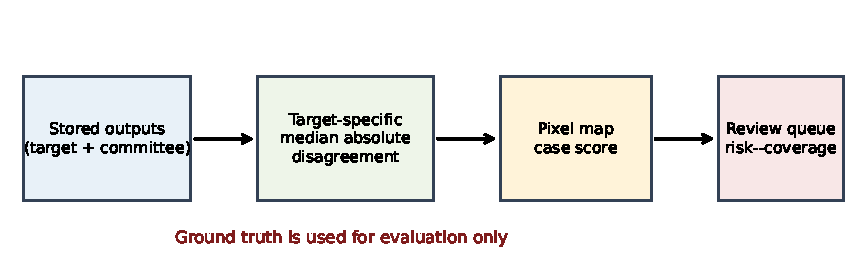
\includegraphics[width=0.96\textwidth]{figure1_framework_compact.pdf}
  \caption{Evaluation framework. Stored target and committee outputs produce a target-specific disagreement map and examination score. The score determines a review queue. Ground truth is hidden from scoring and revealed only for retrospective localization and risk--coverage evaluation.}
  \label{fig:framework}
\end{figure*}

\subsection{Comparators and Committee Tests}

We compare Eq.~\eqref{eq:disagreement} with (i) residuals to linear or cubic interpolation, (ii) a shared committee-dispersion map given by the voxel-wise standard deviation over all available outputs, and (iii) four-view flip TTA variance for SwinIR. We test three committee compositions: all available alternatives, neural peers only, and analytical interpolation only. Finally, each member is removed in turn from the all-member committee. This leave-one-member-out test is performed on pre-aggregated member disagreement scores, so it measures robustness of examination ranking rather than reproducing a new voxel map for every removal.

\subsection{Evaluation}

The absolute reconstruction error is $e_m(i)=|\hat y_m(i)-y(i)|$. Spatial localization is measured by Pearson correlation between $U_m$ and $e_m$ within $M_m$, computed per examination and averaged across cases. All-pixel correlation is a sensitivity analysis. Examination ranking is measured by Spearman correlation between $s_m$ and foreground MAE.

For selective review, examinations are sorted by increasing $s_m$. At coverage $c$, the retained set $A_c$ contains the lowest-score fraction $c$, and risk is
\begin{equation}
 R(c)=\frac{1}{|A_c|}\sum_{j\in A_c} E_j,
\end{equation}
where $E_j$ is examination-level foreground MAE. We report area under this risk--coverage curve (AURC) relative to oracle and random rankings,
\begin{equation}
 \mathrm{nAURC}=\frac{\mathrm{AURC}-\mathrm{AURC}_{\mathrm{oracle}}}
 {\mathrm{AURC}_{\mathrm{random}}-\mathrm{AURC}_{\mathrm{oracle}}}.
 \label{eq:naurc}
\end{equation}
Zero matches the oracle and one matches expected random review. At operating point $c$, relative risk reduction is
\begin{equation}
 \mathrm{RRR}(c)=\frac{R_{\mathrm{random}}-R(c)}{R_{\mathrm{random}}}.
\end{equation}

\section{Experiments}

\subsection{Data and Reconstructors}

We evaluate T2-weighted through-plane interpolation at factor four on IXI \citep{ixi} (115 test examinations), fastMRI-brain \citep{zbontar2018fastmri} (24 examinations), and an external NingXia cross-validation cohort (22 examinations). IXI includes outputs from I$^3$Net, HAT, SwinIR, and a local anatomy-consistency model (ACSI). fastMRI and NingXia include I$^3$Net, HAT, and SwinIR. Linear and cubic interpolation are analytical committee members. All cases in each reported full profile are included; no screening subset contributes to a paper claim.

The datasets differ substantially in intensity scale and acquisition characteristics. Raw AURC is therefore not compared across datasets. nAURC and RRR are scale-normalized ranking measures, while MAE remains dataset-specific. The NingXia result pools held-out predictions across eight folds so each examination is evaluated out of fold.

\subsection{Protocol and Statistics}

All scores are computed from stored NIfTI predictions. For each target model, the all-member committee contains linear, cubic, and every other available neural output. Shapes and case identities must agree before evaluation. Generated slices are identified by the factor-four sampling pattern. The prediction-derived mask in Eq.~\eqref{eq:case-score} is fixed before ground-truth error is examined.

We report point estimates over all cases and use 2,000 paired case-bootstrap replicates for confidence intervals and proxy differences. Failure detection defines the highest-MAE 10\% as failures, but AUROC and AUPRC are secondary because fastMRI and NingXia contain only three positive cases under this definition. The primary endpoints are foreground pixel correlation, case-level Spearman correlation, nAURC, and RRR at 25\%, 50\%, and 75\% coverage.

\section{Results}

\subsection{Disagreement Localizes and Ranks Error}

Table~\ref{tab:main} reports the corrected target-specific score. Across the ten fixed target--dataset evaluations, mean foreground pixel correlation is 0.277--0.519 and case-level Spearman correlation is 0.890--0.966. The 95\% case-bootstrap interval excludes zero for both endpoints in every row. Thus, the spatial result is not created solely by empty background, and high committee disagreement consistently ranks examinations with larger error. Variation across datasets and reconstructors nevertheless argues against interpreting the score as a universal calibrated uncertainty value.

\begin{table*}[t]
  \centering
  \caption{Target-to-all-committee reliability. Pixel $r$ is the mean per-case foreground Pearson correlation; case $\rho$ is Spearman correlation between examination score and MAE. Lower nAURC is better. RRR$_{50}$ is the MAE reduction at 50\% retained coverage relative to random review. Each row is a fixed model--dataset result, not a range over methods.}
  \label{tab:main}
  \begin{tabular}{llrrrr}
\toprule
Dataset & Target & $n$ & Pixel $r$ & Case $\rho$ & nAURC / RRR$_{50}$ \\
\midrule
IXI & ACSI & 115 & 0.435 & 0.954 & 0.035 / 50.1\% \\
 & HAT & 115 & 0.511 & 0.966 & 0.024 / 49.6\% \\
 & I$^3$Net & 115 & 0.351 & 0.951 & 0.044 / 52.1\% \\
 & SwinIR & 115 & 0.519 & 0.965 & 0.025 / 49.5\% \\
fastMRI & HAT & 24 & 0.325 & 0.916 & 0.067 / 19.7\% \\
 & I$^3$Net & 24 & 0.289 & 0.890 & 0.092 / 19.3\% \\
 & SwinIR & 24 & 0.359 & 0.931 & 0.061 / 20.5\% \\
NingXia & HAT & 22 & 0.277 & 0.929 & 0.076 / 22.2\% \\
 & I$^3$Net & 22 & 0.355 & 0.914 & 0.063 / 23.1\% \\
 & SwinIR & 22 & 0.279 & 0.936 & 0.036 / 21.4\% \\
\bottomrule
\end{tabular}

\end{table*}

\subsection{Selective Review Has an Operational Interpretation}

Figure~\ref{fig:risk} compares score-based referral with random and oracle rankings. nAURC is 0.024--0.044 on IXI, 0.061--0.092 on fastMRI, and 0.036--0.076 on NingXia, where zero denotes oracle ranking and one random review. At 50\% coverage, score-based referral lowers retained MAE by 49.5--52.1\%, 19.3--20.5\%, and 21.4--23.1\%, respectively, relative to random review. Every RRR$_{50}$ bootstrap interval excludes zero. Results at 25\%, 50\%, and 75\% coverage are reported directly rather than selecting a favorable test-set operating point.

\begin{figure*}[t]
  \centering
  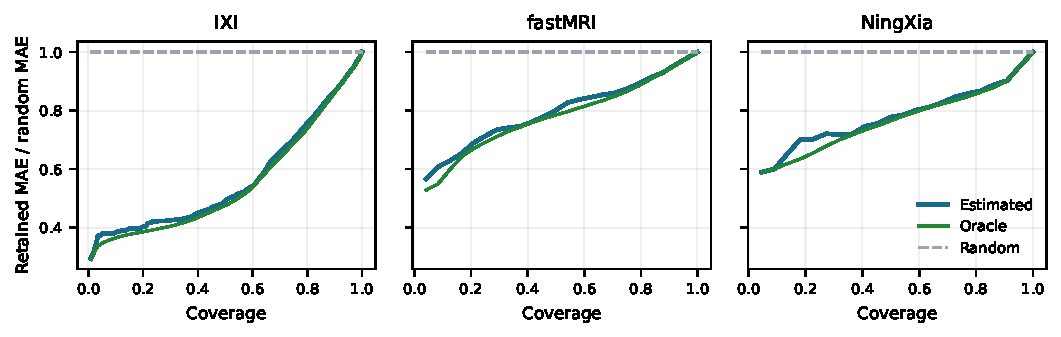
\includegraphics[width=0.96\textwidth]{figure2_committee_risk.pdf}
  \caption{Case-level risk--coverage curves for the all-member target-to-committee score, normalized by the random-review risk and averaged over target reconstructors within each dataset. Lower is better. Oracle and random policies provide interpretable bounds.}
  \label{fig:risk}
\end{figure*}

\subsection{Committee Composition Matters}

Table~\ref{tab:composition} separates neural peers from analytical references. No composition is uniformly best. Mean nAURC for all/neural/analytical committees is 0.032/0.033/0.059 on IXI, 0.073/0.017/0.118 on fastMRI, and 0.058/0.094/0.031 on NingXia. Neural peers therefore carry the strongest ranking signal on fastMRI, whereas analytical references are strongest on NingXia. The all-member committee remains a stable pre-specified default, not an oracle-selected optimum; leave-one-member-out results in the supplement expose individual dependencies.

\begin{table}[t]
  \centering
  \caption{Committee-composition analysis averaged over target reconstructors. Lower nAURC is better; larger RRR$_{50}$ is better.}
  \label{tab:composition}
  \resizebox{\columnwidth}{!}{\begin{tabular}{llrrr}
\toprule
Dataset & Committee & Targets & Case $\rho$ & nAURC / RRR$_{50}$ \\
\midrule
IXI & all & 4 & 0.959 & 0.032 / 50.3\% \\
IXI & neural & 4 & 0.958 & 0.033 / 50.3\% \\
IXI & analytic & 4 & 0.927 & 0.059 / 50.6\% \\
fastMRI & all & 3 & 0.912 & 0.073 / 19.8\% \\
fastMRI & neural & 3 & 0.970 & 0.017 / 21.0\% \\
fastMRI & analytic & 3 & 0.873 & 0.118 / 19.8\% \\
NingXia & all & 3 & 0.926 & 0.058 / 22.2\% \\
NingXia & neural & 3 & 0.883 & 0.094 / 22.2\% \\
NingXia & analytic & 3 & 0.942 & 0.031 / 22.4\% \\
\bottomrule
\end{tabular}
}
\end{table}

The residual comparators are useful but incomplete. A large residual to one analytical interpolation can indicate that the target preserves details absent from that reference, not that the target is wrong. Against shared committee dispersion, target-specific disagreement significantly lowers nAURC for all four IXI targets, is statistically indistinguishable on fastMRI, and is not uniformly better on NingXia. TTA variance remains an auxiliary single-model sensitivity measure: it requires repeated inference and answers a different question from cross-reconstructor disagreement.

\subsection{Failure Modes}

Disagreement is strongest when reconstructors respond differently to difficult content. It can fail when all committee members produce a similar error, and it can over-refer a correct prediction that legitimately differs from conservative analytical interpolation. These two cases correspond to false reassurance and unnecessary review, respectively. Their presence explains why the score should support quality control rather than certify reconstruction correctness.

\begin{figure*}[t]
  \centering
  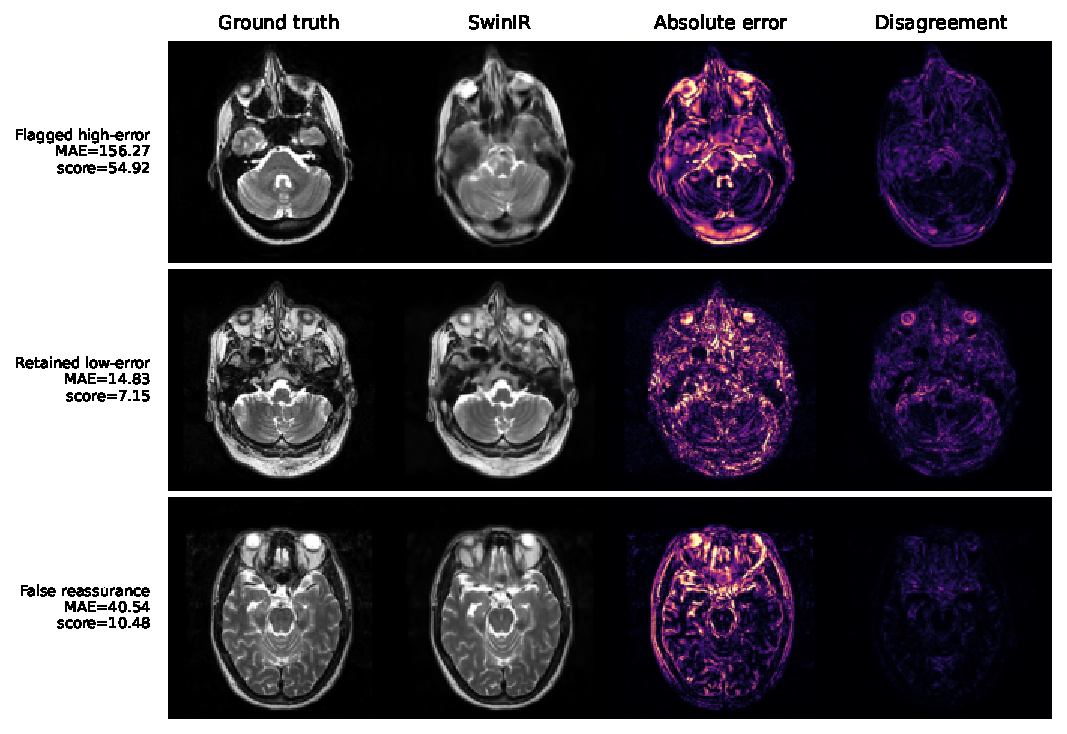
\includegraphics[width=0.94\textwidth]{figure4_committee_qualitative.pdf}
  \caption{Automatically selected IXI examples for SwinIR. Each row uses the generated slice with the largest slice-wise MAE in its examination. The first two rows illustrate a useful referral and a stable retention; the final row exposes a high-error case ranked too confidently. Error and disagreement share a row-wise heat-map scale.}
  \label{fig:qualitative}
\end{figure*}

\section{Discussion}

The study supports a narrow but practical conclusion: heterogeneous reconstruction outputs contain information about where and when an interpolation result is likely to be inaccurate. The evidence is strongest when assessed as a ranking problem. Pixel correlation tests localization, case Spearman tests triage, and risk--coverage analysis translates the score into a review workload. Reporting all three prevents a background-dominated map or a small set of easily separated failures from carrying the entire claim.

The corrected target-specific definition is important. A single standard-deviation map computed from all outputs is a property of the committee, not of a particular target model. Equation~\eqref{eq:disagreement} instead asks how far the target lies from alternatives and explicitly excludes self-comparison. The committee-composition analysis then reveals whether the score is driven by neural peers, analytical references, or both.

The method is complementary to probabilistic uncertainty. It is attractive when several predictions have already been generated, when model internals are unavailable, or when a common retrospective audit is needed across architectures. It is less attractive when only one reconstructor can be run, in which case TTA, learned uncertainty, reconstruction residuals, or acquisition-aware methods may be more appropriate.

\paragraph{Limitations.}
First, committee disagreement cannot detect errors shared by all members and may be weaker when committee architectures or training data are highly correlated. Second, running several reconstructors is not free if their outputs do not already exist; our study measures post-hoc scoring cost, not the cost of creating the committee. Third, the external cohorts are small, particularly for binary failure analysis, and confidence intervals should be interpreted accordingly. Fourth, foreground masks are intensity-based and do not isolate clinically important anatomy or pathology. Fifth, reconstruction error is not equivalent to diagnostic harm. No reader study or downstream clinical task is included, so the protocol does not establish clinical safety.

\section{Conclusion}

We presented a ground-truth-free reliability-ranking protocol for MRI through-plane interpolation. A target-specific median disagreement map can be computed from heterogeneous reconstruction outputs, aggregated into an examination score, and evaluated through spatial error association and selective risk. Across three T2 MRI cohorts, the score provides a useful but imperfect review signal. Its value lies in prioritizing inspection of existing reconstructions; it is neither a calibrated probability nor a guarantee that consensus is correct.

\bibliographystyle{plainnat}
\bibliography{references}

\end{document}
